
\documentclass[tikz, border=10pt]{standalone}

\usepackage{tikz}
\usetikzlibrary{positioning, fit, calc, shapes, arrows.meta, decorations.pathreplacing, shadows, quotes, angles}
\usepackage{tikz-3dplot}

\begin{document}

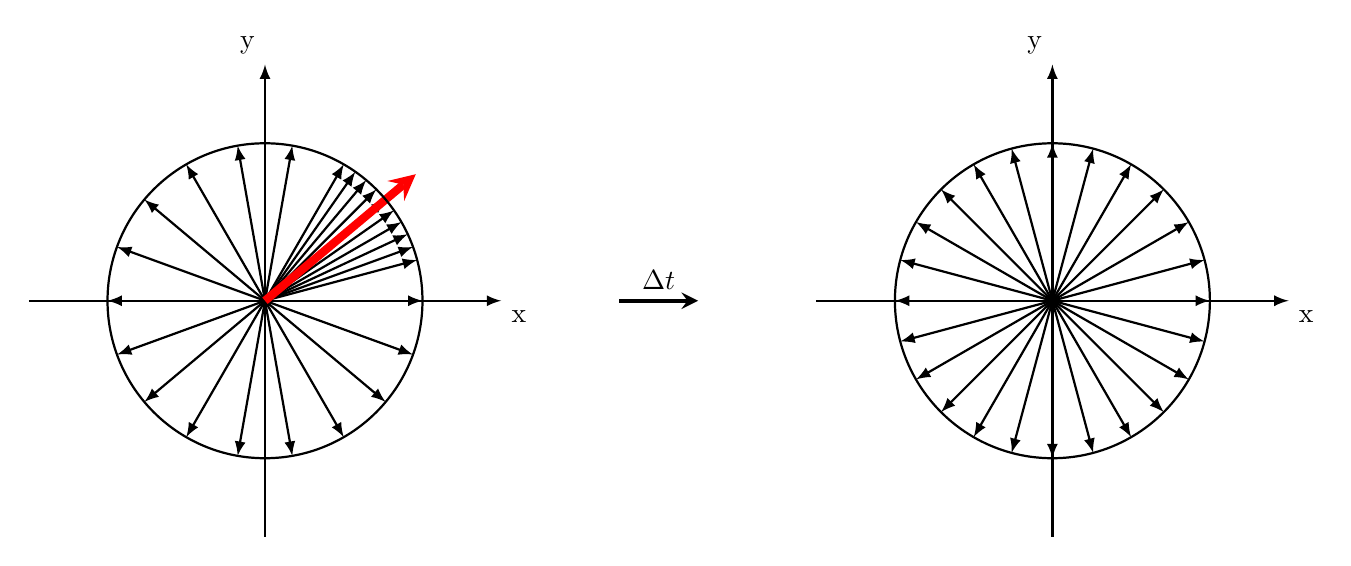
\begin{tikzpicture}[>=latex]

\draw[thick,->] (-3,0) -- (3,0) node[anchor=north west] {x};
\draw[thick,->] (0,-3) -- (0,3) node[anchor=south east] {y};

\foreach \x in {20,40,...,360,375,385,390,395,405,410,415} {
        \draw[thick,->] (0,0) coordinate (O) -- (\x:2) coordinate (oc) 
node[midway,below] {};

}

\draw[red, line width=3pt, -stealth] (0,0) coordinate (O) -- (40:2.5) coordinate (oc) 
node[midway,below] {};
 \draw[black, thick] (O) circle (2 cm);

\path[draw,ultra thick,-stealth] (4.5,0) -- (5.5,0)node[midway, above]{$\Delta t$} node[below,midway]{};

\begin{scope}[xshift=10cm]

\draw[thick,->] (-3,0) -- (3,0) node[anchor=north west] {x};
\draw[thick,->] (0,-3) -- (0,3) node[anchor=south east] {y};

\foreach \x in {15,30,...,360} {
        \draw[thick,->] (0,0) coordinate (O) -- (\x:2) coordinate (oc) 
node[midway,below] {};
}
 \draw[black, thick] (O) circle (2 cm);

\end{scope}

% \draw[thick,->] (-3+10,0) -- (3+10,0) node[anchor=north west] {x};
% \draw[thick,->] (0+10,-3) -- (0+10,3) node[anchor=south east] {y};
% % \draw[black, thick] (1O) circle (2 cm);

%  \foreach \x in {15,30,45,...,360} {
%          \draw[thick,->] (10,0) coordinate (K) -- (\x:2) {};
        
% }
%  \draw[black, thick] (K) circle (2 cm);


\end{tikzpicture}


% \begin{tikzpicture}[remember picture]
% \tikzset{puls/.style={
%     rectangle, draw=black, very thick, fill=gray!30 ,minimum width=1cm,minimum height=2cm
%     }
% }

%     \coordinate (start) at (0, 0);
%     \coordinate (end) at (8.5, 0);
    
%     \coordinate (rf_1) at ($(start) + (3,0)$);
%     \coordinate (rf_2) at ($(rf_1) + (3,0)$);
   
    
    
%     \coordinate (del_1) at ($(1.5,0.5)$);
%     \coordinate (del_2) at ($(del_1) + (3,0)$);
%     \coordinate (del_3) at ($(del_2) + (3,0)$);
%      \coordinate (signal) at ($(del_3) + (3,0)$);  
      
%     \path (rf_1) node[puls, above, label= \LARGE$\frac{\pi}{2}$]{\LARGE x};
%      \path (rf_1)  node[below,label={[label distance=0 cm]below:{\LARGE $P_1$}} ]{};
   
%     \path (rf_2) node[puls,above, label= \LARGE$\frac{\pi}{2}$ ]{\LARGE x};
%      \path (rf_2)  node[below,label={[label distance=0 cm]below:{\LARGE $P_1$}} ]{};
    
%     \draw  (del_1) node[above, label= \LARGE $D_1$] {};
%     \draw  (del_2) node[above, label= \LARGE $D_6$] {};
%     \draw  (del_3) node[above, label= \LARGE $D_7$] {};
%     \draw  (signal) node[above, label= \LARGE $D_w$] {};

  
%      \draw[very thick] ($(start)$ ) -- ( $(end)$ ) node[label={[label distance=-5.5 cm]left:{\large $t$}}, anchor = north] {};
%       \def\a{-1}
%     \def\b{10}
%     \def\c{2}
%     \def\N{1000}
%     \draw[very thick,samples=\N,variable=\t, domain=0:5,-stealth] (signal) plot({\t+ 8.5 },  {exp(\a * \t)*\c*sin( \b*\t r)} );

% \end{tikzpicture}


\end{document}

